\section{Arquitectura y tecnologías de una aplicación web}
\label{sec:arquitectura_sistema}

En el mundo del software existen dos tipos de aplicaciones: las aplicaciones de escritorio y las aplicaciones web. Las aplicaciones de escritorio son aquellas que se instalan en un ordenador y se ejecutan de forma local, mientras que las aplicaciones web son aquellas que se ejecutan en un servidor y se acceden a través de un navegador web.

Desde los inicios del desarrollo de software, las aplicaciones de escritorio han sido la norma. Sin embargo, en los últimos años ha habido un cambio significativo hacia el desarrollo de aplicaciones web, pues el avance de las distintas tecnologías web y la conectividad a internet han mitigado considerablemente las desventajas que anteriormente presentaban. \cite{evo_web}

Las aplicaciones de escritorio no requieren de un servidor externo para funcionar, toda la lógica se encuentra en el ordenador del usuario y es este mismo quien lo ejecuta. Esto hace que la aplicación sea más rápida y eficiente, ya que no hay necesidad de enviar datos a través de internet. No obstante, esto también significa que el usuario debe instalar la aplicación en su ordenador y mantenerla actualizada, lo que puede ser un inconveniente. \cite{web_vs_desktop}

Por otro lado, las aplicaciones web sí que requieren de un servidor externo para funcionar. Esto significa que el usuario no necesita instalar nada en su ordenador, ya que la aplicación se ejecuta en el servidor y se accede a través de un navegador web. Este paradigma de desarrollo permite que la aplicación sea más accesible, pues se puede acceder a la aplicación desde cualquier dispositivo y lugar con conexión a internet. Además, como todo se encuentra en el servidor y no en el usuario, las actualizaciones son mucho más inmediatas. Sin embargo, esto también significa que la aplicación puede ser más lenta y menos eficiente debido a que la lógica y los datos no se encuentran en el ordenador del usuario, sino en el servidor. \cite{web_vs_desktop}

La mejor conectividad a internet y el avance de las tecnologías web han permitido que las aplicaciones web sean cada vez más rápidas y eficientes. Esto ha llevado a un aumento en la popularidad de las aplicaciones web, y muchas empresas están optando por desarrollar aplicaciones web en lugar de aplicaciones de escritorio.

\subsection{Arquitectura y tecnologías}

La arquitectura de una aplicación web se refiere a la forma en que se organiza y estructura el software. Esto incluye la forma en que se comunican los diferentes componentes de la aplicación, así como la forma en que se almacenan y gestionan los datos. Todas las aplicaciones web están compuestas por tres componentes principales: el cliente, la lógica de negocio y la base de datos.

Estos tres componentes se dividen en dos bloques: el \textit{frontend} y el \textit{backend}. El \textit{frontend} es la parte de la aplicación que interactúa con el usuario, es decir, el cliente, mientras que el \textit{backend} es la parte de la aplicación que se encarga de gestionar los datos y la lógica de negocio. Ambos bloques se comunican entre sí a través de una API (Interfaz de Programación de Aplicaciones), que es un conjunto de reglas y protocolos que permiten que diferentes componentes de software se comuniquen entre sí. Todo esto se puede ver en la figura \ref{fig:arquitectura_web}.

\begin{figure}
    \centering
    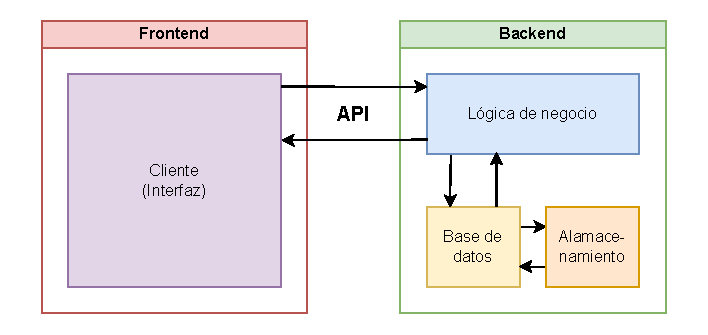
\includegraphics[width=0.8\textwidth]{figures/theoric_frame/arquitectura_web.pdf}
    \caption{Arquitectura de una aplicación web.}
    \label{fig:arquitectura_web}
\end{figure}

\subsubsection{\textit{Frontend}}

El \textit{frontend} es la parte de la aplicación que interactúa con el usuario. Esto incluye la interfaz de usuario, que es la parte de la aplicación que el usuario ve y con la que interactúa, así como la lógica de presentación, que es la parte de la aplicación que se encarga de mostrar los datos al usuario. El \textit{frontend} se desarrolla principalmente utilizando HTML, CSS y JavaScript, tecnologías que se ejecutan de manera nativa en los navegadores.

El HTML (\textit{Hypertext Markup Language}) es el lenguaje de marcado utilizado para estructurar el contenido de una página web. El CSS (\textit{Cascading Style Sheets}) es el lenguaje utilizado para dar estilo a una página web, es decir, para definir cómo se verá el contenido estructurado por el HTML. Por último, JavaScript es un lenguaje de programación que se utiliza para añadir interactividad a una página web, es decir, para permitir que el usuario interactúe con la aplicación.

Con todo esto, el servidor envía todo este contenido al usuario de manera que su navegador lo pueda representar, en caso del HTML y el CSS, y ejecutar, en caso del JavaScript.

\textcolor{red}{AFEGIR EXPLICACIÓ REACT}

\subsubsection{\textit{Backend}}

\subsubsection{API}

\begin{figure}
    \centering
    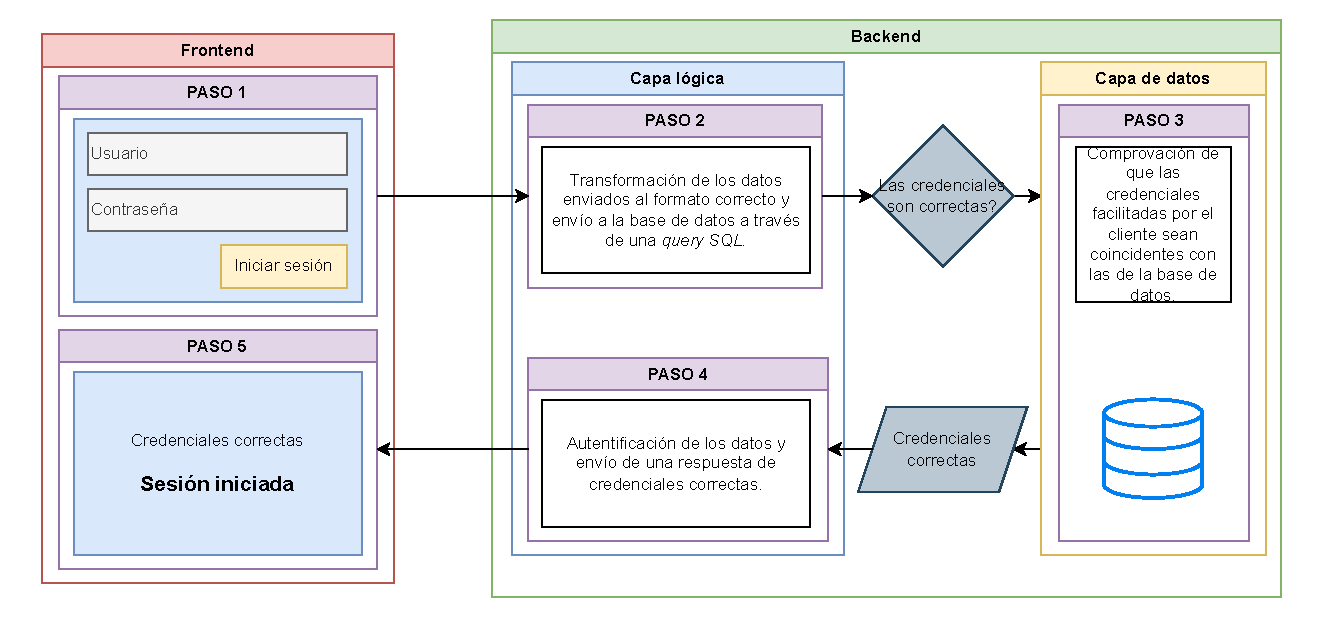
\includegraphics[width=0.8\textwidth]{figures/theoric_frame/use_case.pdf}
    \caption{Diagrama de flujo del proceso de autenticación de usuario como caso de uso.}
    \label{fig:use_case}
\end{figure}

\subsection{Tecnologías web}